\begin{titlepage}.
    \begin{tikzpicture}[remember picture,overlay]

% UTT Background under the title and info box
\coordinate [right=8mm, below=80mm] (uttbackground_anchor) at (current page.north west);
\node [name=uttsquare,anchor=north west] at (uttbackground_anchor){
%\includegraphics[width=19.4cm]{first-page-background.png}};
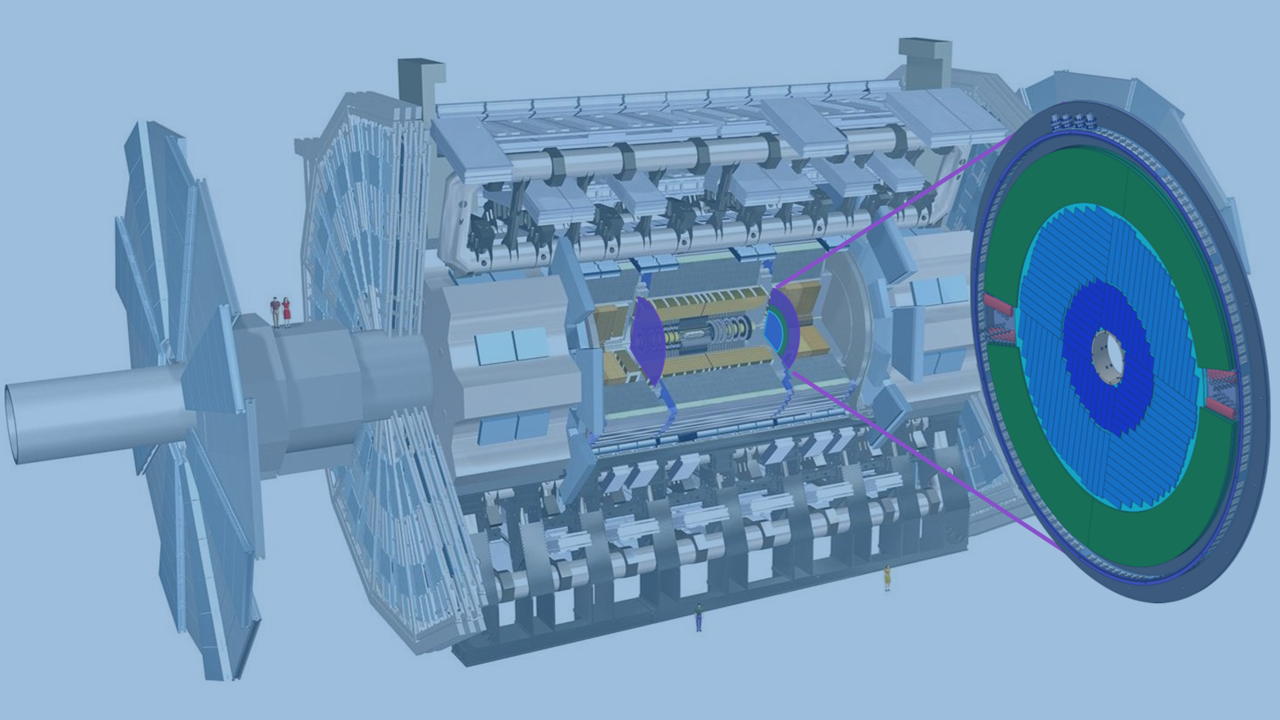
\includegraphics[width=19.4cm]{assets/ATLAS_BACKGROUND.png}};

\end{tikzpicture}

    % Margin to begin the text under the uttsquare
    \vspace{3.5cm}

    
    % Authhor
    \begin{textblock*}{15cm}(3cm,2.cm)
        \makeatletter
        \begin{huge}
            \begin{center}
                \color{black}
                 Renato Aparecido Negrão de Oliveira\\ 
            \end{center}
         \end{huge}
     
    \end{textblock*}
    
    %TITLE
    \begin{textblock*}{15cm}(3cm,12cm)
        \begin{Huge}
            \begin{center}
                \makeatletter
                \noindent\textcolor{white}{Desenvolvimento de um detector de silício frontal para a medida de trajetórias e tempo no experimento ATLAS-LHC}
                \makeatother
            \end{center}
        \end{Huge}
    \end{textblock*}

    % Info box
    \begin{textblock*}{15cm}(2.5cm,20cm)
        \makeatletter
        \begin{LARGE}
            \setcellgapes{4pt}
            \makegapedcells
            {\color{black}\begin{tabularx}{15cm}{XX}
                \textbf{Supervisor :} Dr. Marco Aurélio Lisboa Leite (IFUSP)\\ 
                \textbf{Supervisor :} Dr. Marcelo Gameiro Munhoz (IFUSP)
            \end{tabularx}}
        \end{LARGE}
        \makeatother
    \end{textblock*}
    
    % FOOT NOTE
    \begin{textblock*}{15cm}(3cm,24cm)
        \makeatletter
        \begin{center}
            {\color{black}
                \textbf{SÃO, PAULO 2019} 
            }
        \end{center}
        \makeatother
    \end{textblock*}

\end{titlepage}

